\appendix
\section{Abundance Plane of All Simulations}\label{app:allmerge}
We show summary plots of the abundance planes of all simulations in our orbital grid in Figures~\ref{fig:allmerge0} to \ref{fig:allmerge8}.

\begin{figure*}
  \centering
  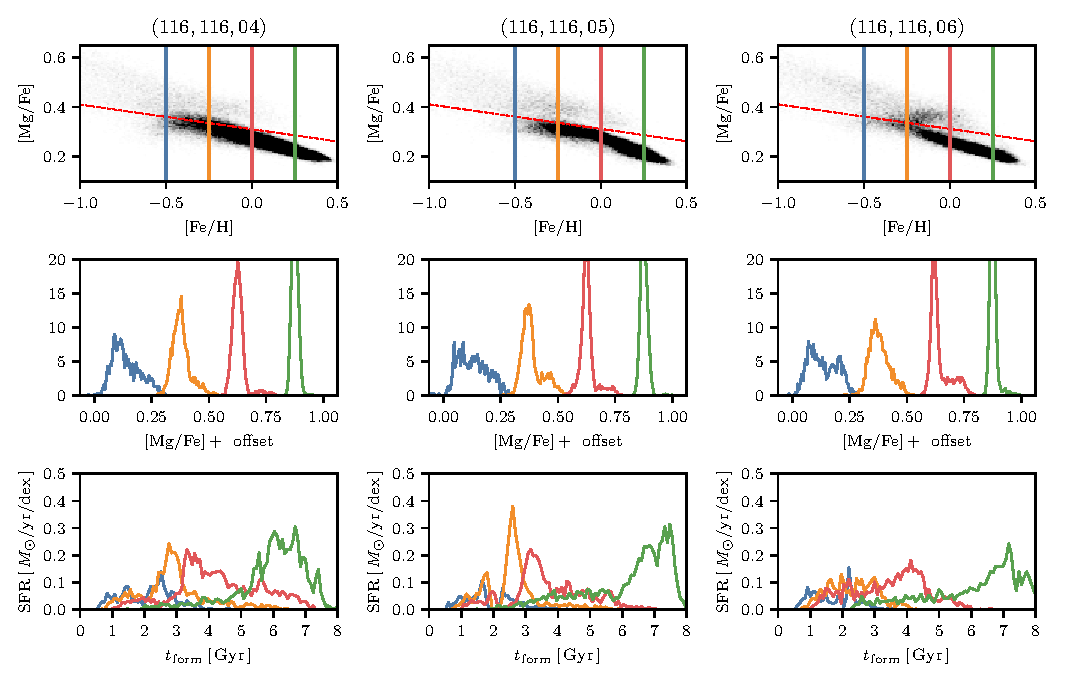
\includegraphics[width=\textwidth]{allmerge/allmerge0.pdf}
  \caption{A summary of the abundance plane and star formation history of all simulations within the orbital grid. Each figure shows the outcome of a simulation at a fixed $R_0$ and $V_0$, varying $\eta$. The title of each column shows the $R_0$, $V_0$, and $\eta$ of that simulation, in order. The upper and middle rows replicate Figure~\ref{fig:fig1}, which show the distribution of stars in the abundance plane of \MgFe{}-\FeH{} as well as 1D histograms at a fixed \FeH{} of $-0.5$, $-0.25$, $0$, and $0.25$. The lower rows replicate Figure~\ref{fig:before_after_sfh_by_iron}, showing the star formation history at each \FeH{}.}
  \label{fig:allmerge0}
\end{figure*}

\begin{figure*}
  \centering
  \includegraphics[width=\textwidth]{allmerge/allmerge1.pdf}
  \caption{A continuation of Figure~\ref{fig:allmerge0}.}
  \label{fig:allmerge1}
\end{figure*}

\begin{figure*}
  \centering
  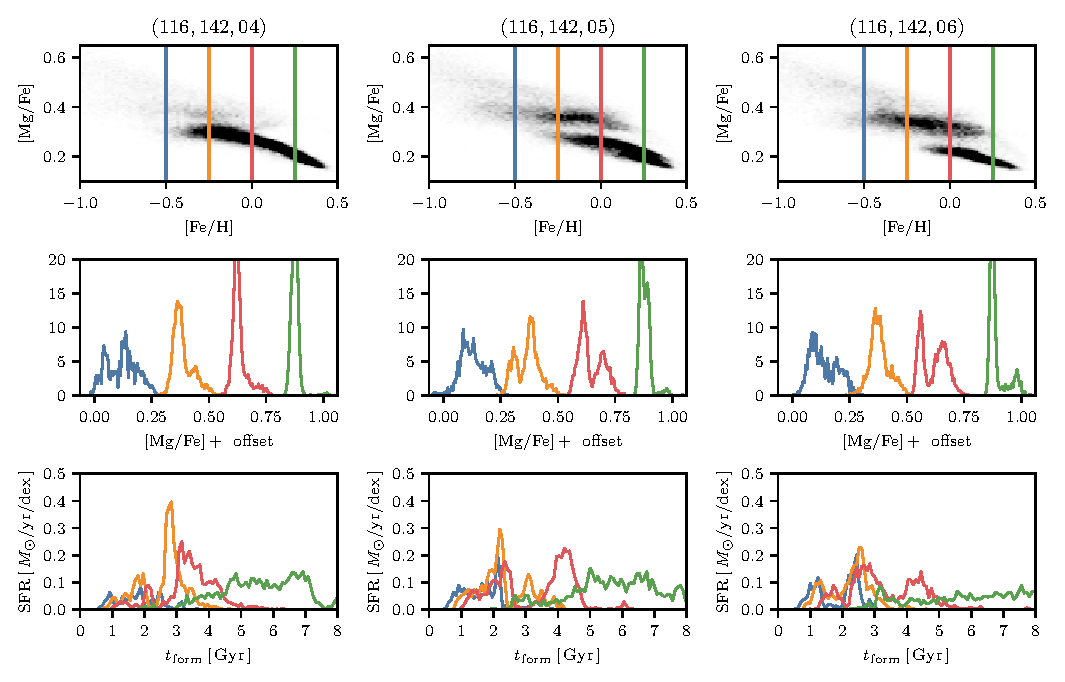
\includegraphics[width=\textwidth]{allmerge/allmerge2.pdf}
  \caption{A continuation of Figure~\ref{fig:allmerge0}.}
  \label{fig:allmerge2}
\end{figure*}

\begin{figure*}
  \centering
  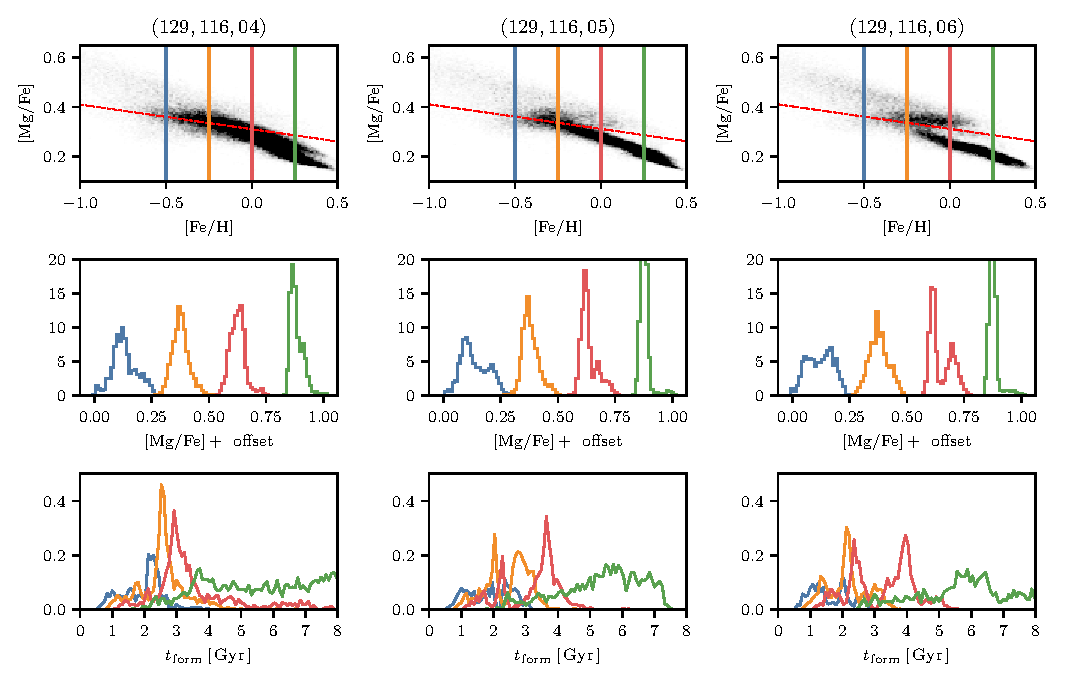
\includegraphics[width=\textwidth]{allmerge/allmerge3.pdf}
  \caption{A continuation of Figure~\ref{fig:allmerge0}.}
  \label{fig:allmerge3}
\end{figure*}

\begin{figure*}
  \centering
  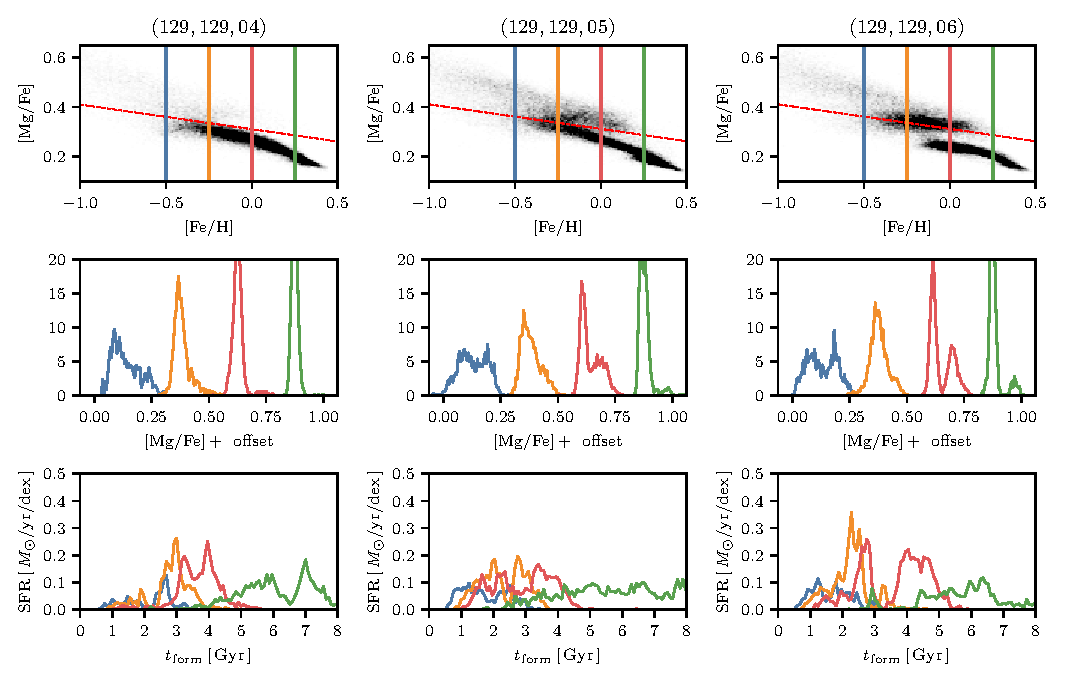
\includegraphics[width=\textwidth]{allmerge/allmerge4.pdf}
  \caption{A continuation of Figure~\ref{fig:allmerge0}.}
  \label{fig:allmerge4}
\end{figure*}

\begin{figure*}
  \centering
  \includegraphics[width=\textwidth]{allmerge/allmerge5.pdf}
  \caption{A continuation of Figure~\ref{fig:allmerge0}.}
  \label{fig:allmerge5}
\end{figure*}

\begin{figure*}
  \centering
  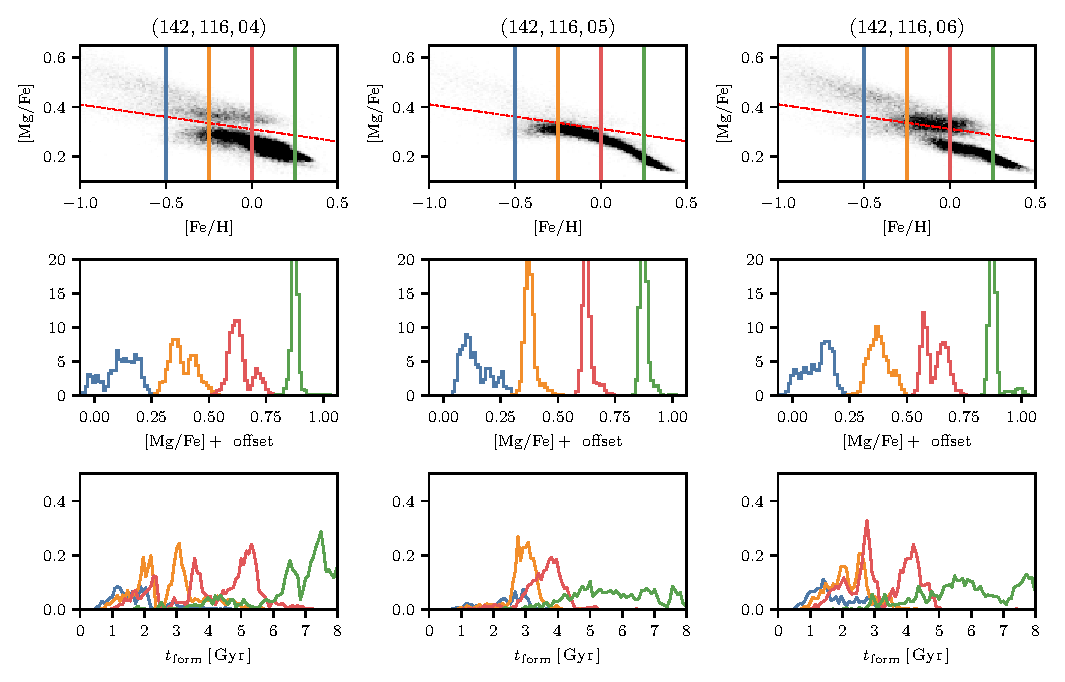
\includegraphics[width=\textwidth]{allmerge/allmerge6.pdf}
  \caption{A continuation of Figure~\ref{fig:allmerge0}.}
  \label{fig:allmerge6}
\end{figure*}

\begin{figure*}
  \centering
  \includegraphics[width=\textwidth]{allmerge/allmerge7.pdf}
  \caption{A continuation of Figure~\ref{fig:allmerge0}.}
  \label{fig:allmerge7}
\end{figure*}

\begin{figure*}
  \centering
  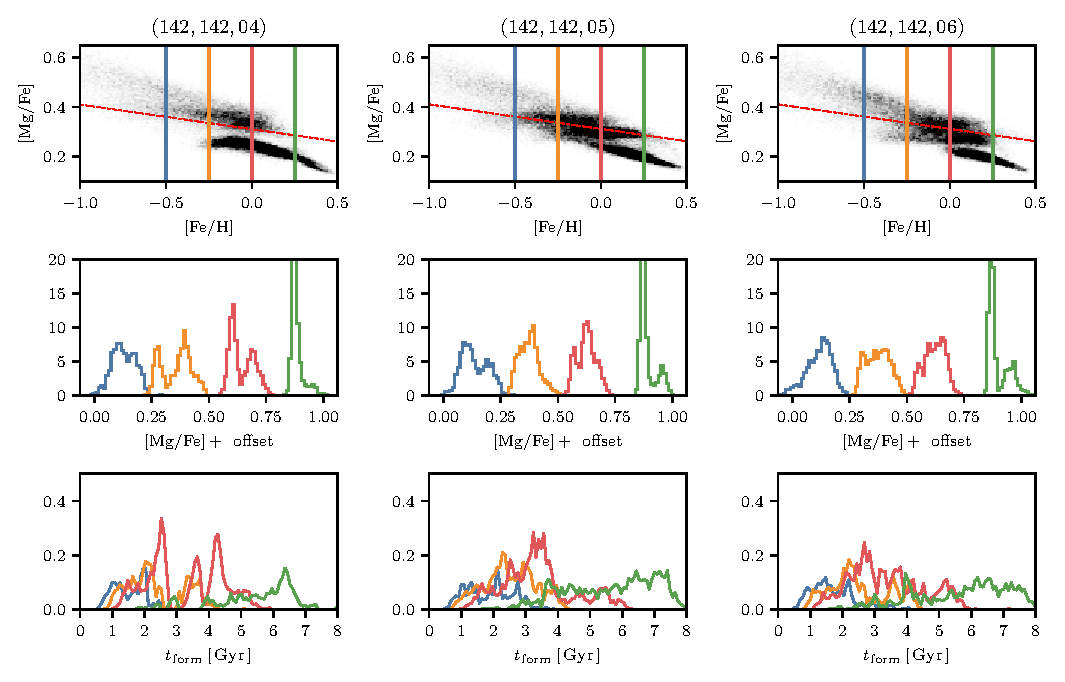
\includegraphics[width=\textwidth]{allmerge/allmerge8.pdf}
  \caption{A continuation of Figure~\ref{fig:allmerge0}.}
  \label{fig:allmerge8}
\end{figure*}

\section{Cause of Suppressed Star Formation}\label{app:cause_qui}

\begin{figure*}
  \centering
  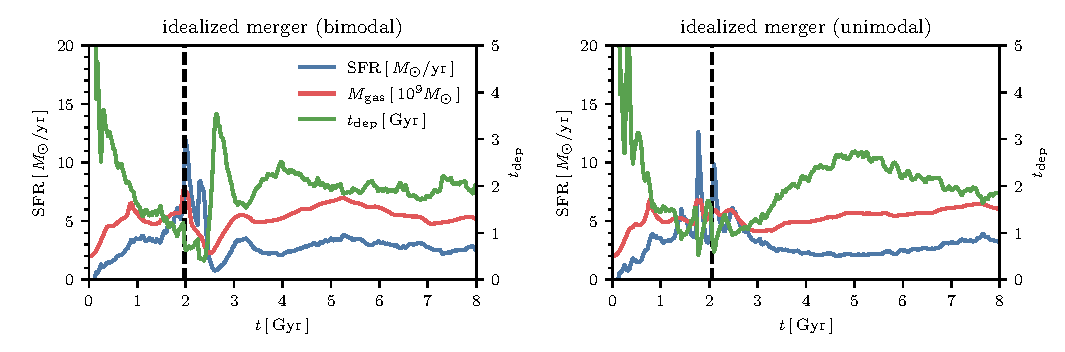
\includegraphics[width=\textwidth]{SFR_Mgas_tdep.pdf}
  \caption{\textbf{The suppression of star formation in the bimodal simulation is associated with both a reduction in gas mass as well as an increase in the depletion time.} The drop in star formation (blue line) at $\sim2.5-3\,\Gyr$ is associated with both a reduction in the total gas mass (red line) as well as an increase in the depletion time (green line). This shows that the SFR suppression is a result of both less gas mass and more inefficient star formation.}
  \label{fig:SFR_Mgas_tdep}
\end{figure*}

\begin{figure}
  \centering
  \includegraphics[width=242.26653pt]{MdotBH_rsep.pdf}
  \caption{\textbf{The bimodal merger is associated with high accretion rates onto the central SMBH.} Around the time of each pericentric passage, and slightly after, the accretion rate (blue line) becomes very high. Here, it is shown as a fraction of the Eddington accretion rate. During the merger, the accretion rate reaches as high as Eddington at some times, but is always above $10\%$. The orbital separation between the central and satellite is shown in the orange line.}
  \label{fig:MdotBH_rsep}
\end{figure}